% ── Chương 6: Bipartite Ranking ──────────────────────────────────────────────
\subsection{Bipartite Ranking}
\label{sec:bipartite}

\subsubsection{Thiết lập Bài toán (Setting)}

Trong bài toán phân hạng nhị phân (\textit{bipartite ranking}), tập mẫu đầu vào $\Xcal$ được phân hoạch thành hai lớp riêng biệt:
\begin{itemize}
    \item $\Xcal^+$: lớp tích cực (\textit{positive} - ví dụ: tài liệu liên quan).
    \item $\Xcal^-$: lớp tiêu cực (\textit{negative} - ví dụ: tài liệu không liên quan).
\end{itemize}
Nhiệm vụ cốt lõi: học một hàm số cho điểm (scoring function) $h: \Xcal \to \R$ sao cho mọi phần tử lớp tích cực luôn được xếp hạng \textbf{cao hơn} mọi phần tử lớp tiêu cực.

\textbf{Khác biệt cấu trúc so với score-based setting tổng quát:}
\begin{itemize}
    \item Thay vì có một phân phối xác suất chung $D$ trên các cặp, không gian bipartite được đặc trưng bởi \textit{hai phân phối xác suất độc lập}: $D^+$ trên $\Xcal^+$ và $D^-$ trên $\Xcal^-$.
    \item Mẫu dữ liệu huấn luyện gồm hai tập riêng biệt:
          $S^+ = (x'_1, \ldots, x'_m)$ được lấy mẫu i.i.d. từ $D^+$,
          $S^- = (x_1, \ldots, x_n)$ được lấy mẫu i.i.d. từ $D^-$.
    \item Tất cả $mn$ cặp tích cực - tiêu cực $(x'_i, x_j)$ đều được đưa vào đánh giá lỗi.
\end{itemize}

\subsubsection{Generalization error và empirical error}

\begin{definition}{Bipartite Misranking Error}{bipartite_R}
Sai số phân hạng nhị phân tổng quát $R(h)$ được định nghĩa là xác suất một phần tử dương bị xếp thấp hơn phần tử âm:
\begin{equation}
    R(h) = \Prob_{\substack{x \sim D^- \\ x' \sim D^+}}\bigl[h(x') < h(x)\bigr].
    \label{eq:R_bipartite}
\end{equation}
Sai số thực nghiệm tương ứng trên tập huấn luyện $S^+, S^-$ là tỷ lệ các cặp bị xếp sai:
\begin{equation}
    \hat{R}_{S^+, S^-}(h) = \frac{1}{mn} \sum_{i=1}^m \sum_{j=1}^n \mathbf{1}_{h(x'_i) < h(x_j)}.
    \label{eq:R_emp_bipartite}
\end{equation}
\end{definition}

\begin{tcolorbox}[colback=red!5, colframe=red!50!black,
                 title={Khác biệt bản chất với binary classification}]
Mặc dù cùng làm việc trên hai tập nhãn (positive/negative), \textbf{bipartite ranking không phải là classification}. 
Lý do nằm ở mục tiêu tối ưu hóa:
\begin{itemize}
    \item \textbf{Classification}: Đưa ra quyết định tuyệt đối (pointwise) cho từng điểm độc lập: $h(x) > 0$ với mẫu dương, $h(x) < 0$ với mẫu âm.
    \item \textbf{Bipartite ranking}: Tập trung vào quan hệ so sánh tương đối (pairwise) giữa các cặp: $h(x') > h(x)$.
\end{itemize}
Một bộ phân lớp tốt (error 0\%) chắc chắn sẽ là một bộ phân hạng hoàn hảo, nhưng điều ngược lại hoàn toàn không đúng: một bộ phân hạng có năng lực phân tách tốt (AUC rất cao) vẫn có thể có sai số classification cực tệ nếu ta chọn ngưỡng tuyệt đối $\theta$ cắt ngang phân bố không phù hợp.
\end{tcolorbox}

\subsubsection{Vấn đề hiệu năng tính toán: Thách thức $mn$ cặp}

Áp dụng SVM Ranking trực tiếp vào bipartite setting yêu cầu tối ưu hóa hệ thống ràng buộc với $mn$ biến slack. Với kích thước dữ liệu thực tế trung bình $m = n = 1000$, ta phải xử lý tới **một triệu biến slack** -- một thách thức cực lớn làm cạn kiệt tài nguyên RAM và thời gian CPU. Thuật toán RankBoost giải quyết triệt để thách thức này nhờ tính chất phân tích nhân tử đặc biệt dưới đây.

\subsubsection{BipartiteRankBoost: Độ phức tạp tuyến tính $\mathcal{O}(m+n)$}

\textbf{Tính chất tách nhân tử then chốt}: Hàm tổn thất lũy thừa của RankBoost cho phép phân tách hàm mục tiêu toàn cục thành tích của hai hàm thành phần độc lập:
\begin{align}
    F_{\text{RankBoost}}(\bm{\alpha})
    &= \sum_{i=1}^m \sum_{j=1}^n \exp\bigl(-[f(x'_i) - f(x_j)]\bigr) \nonumber \\
    &= \biggl(\sum_{i=1}^m e^{-f(x'_i)}\biggr) \biggl(\sum_{j=1}^n e^{f(x_j)}\biggr) \nonumber \\
    &= F^+(\bm{\alpha}) \cdot F^-(\bm{\alpha}).
    \label{eq:F_factor}
\end{align}
Hệ quả trực tiếp là phân phối cặp $D_t$ cũng được phân tách độc lập:
\[
    D_t(i, j) = D^+_t(i) \cdot D^-_t(j),
\]
với phân phối biên ban đầu đều: $D^+_1(i) = 1/m$, $D^-_1(j) = 1/n$.

\begin{lemma}{Tách phân phối trong BipartiteRankBoost}{factor_dist}
Tính chất phân tích độc lập của phân phối biên được bảo toàn nghiêm ngặt qua các vòng boosting thích ứng:
\begin{equation}
    D_{t+1}(i, j) = \frac{D^+_t(i) e^{-\alpha_t h_t(x'_i)}}{Z^+_t} \cdot \frac{D^-_t(j) e^{\alpha_t h_t(x_j)}}{Z^-_t},
\end{equation}
với các hằng số chuẩn hóa biên độc lập:
\[
    Z^+_t = \sum_{i=1}^m D^+_t(i) e^{-\alpha_t h_t(x'_i)}, \quad
    Z^-_t = \sum_{j=1}^n D^-_t(j) e^{\alpha_t h_t(x_j)}.
\]
\end{lemma}

\begin{proof}[Chứng minh tự bổ sung chi tiết]
Áp dụng công thức cập nhật phân phối cặp RankBoost gốc:
\[
    D_{t+1}(i, j) = \frac{D_t(i, j) e^{-\alpha_t [h_t(x'_i) - h_t(x_j)]}}{Z_t}.
\]
Thế giả thiết quy nạp $D_t(i,j) = D^+_t(i) D^-_t(j)$ và khai triển hàm mũ:
\[
    e^{-\alpha_t[h_t(x'_i) - h_t(x_j)]} = e^{-\alpha_t h_t(x'_i)} \cdot e^{\alpha_t h_t(x_j)},
\]
ta có thể phân tách hằng số chuẩn hóa toàn cục $Z_t$:
\[
    Z_t = \sum_{i=1}^m \sum_{j=1}^n D^+_t(i) D^-_t(j) e^{-\alpha_t h_t(x'_i)} e^{\alpha_t h_t(x_j)}
    = \left( \sum_{i=1}^m D^+_t(i) e^{-\alpha_t h_t(x'_i)} \right) \left( \sum_{j=1}^n D^-_t(j) e^{\alpha_t h_t(x_j)} \right)
    = Z^+_t \cdot Z^-_t.
\]
Thế ngược $Z_t = Z^+_t Z^-_t$ vào biểu thức cập nhật $D_{t+1}(i,j)$, ta thu được:
\[
    D_{t+1}(i, j) = \left( \frac{D^+_t(i) e^{-\alpha_t h_t(x'_i)}}{Z^+_t} \right) \cdot \left( \frac{D^-_t(j) e^{\alpha_t h_t(x_j)}}{Z^-_t} \right).
\]
Bổ đề được chứng minh hoàn tất.
\end{proof}

\textbf{Hệ quả cách mạng}: Thay vì phải duy trì và cập nhật một ma trận phân phối kích thước khổng lồ $D_t \in \R^{mn}$, thuật toán chỉ cần lưu trữ hai vector biên kích thước nhỏ $D^+_t \in \R^m$ và $D^-_t \in \R^n$. Biên lỗi của base ranker được tính siêu nhanh qua hiệu hai kỳ vọng biên:
\begin{equation}
    \E_{(i,j) \sim D_t}[h(x'_i) - h(x_j)] = \E_{i \sim D^+_t}[h(x'_i)] - \E_{j \sim D^-_t}[h(x_j)] = \epsilon^+_t - \epsilon^-_t.
\end{equation}
Độ phức tạp tính toán cho mỗi vòng boosting được tối ưu hóa từ **bậc hai $\mathcal{O}(mn)$ xuống tuyến tính $\mathcal{O}(m+n)$**, tạo điều kiện cho RankBoost chạy cực nhanh trên các tập dữ liệu lớn.

Sự cải tiến vượt trội này được hệ thống hóa qua thuật toán chi tiết dưới đây:

\begin{algorithm}[H]
\caption{BipartiteRankBoost}
\label{alg:bipartite_rankboost}
\begin{algorithmic}[1]
\REQUIRE Mẫu tích cực $S^+ = (x'_1, \ldots, x'_m)$ và mẫu tiêu cực $S^- = (x_1, \ldots, x_n)$
\STATE Khởi tạo phân phối biên: $D^+_1(i) = 1/m$ với mọi $i \in [m]$; $D^-_1(j) = 1/n$ với mọi $j \in [n]$
\FOR{$t = 1$ to $T$}
    \STATE Chọn $h_t \leftarrow \displaystyle\arg\max_{h \in \Hcal} \left( \E_{i \sim D^+_t}[h(x'_i)] - \E_{j \sim D^-_t}[h(x_j)] \right)$
    \STATE Tính hệ số tin cậy: $\alpha_t \leftarrow \frac{1}{2}\log\dfrac{\epsilon^+_t}{\epsilon^-_t}$ \quad với $\epsilon^+_t = \E_{i \sim D^+_t}[h_t(x'_i)]$ và $\epsilon^-_t = \E_{j \sim D^-_t}[h_t(x_j)]$
    \STATE Tính các hằng số chuẩn hóa biên dạng đóng (cho base ranker nhị phân $\{0,1\}$):
           $$Z^+_t \leftarrow 1 - \epsilon^+_t + \sqrt{\epsilon^+_t \epsilon^-_t}$$
           $$Z^-_t \leftarrow 1 - \epsilon^-_t + \sqrt{\epsilon^+_t \epsilon^-_t}$$
    \STATE Cập nhật phân phối biên thích ứng:
           $$D^+_{t+1}(i) \leftarrow \frac{D^+_t(i) e^{-\alpha_t h_t(x'_i)}}{Z^+_t}$$
           $$D^-_{t+1}(j) \leftarrow \frac{D^-_t(j) e^{\alpha_t h_t(x_j)}}{Z^-_t}$$
\ENDFOR
\RETURN $f = \sum_{t=1}^T \alpha_t h_t$
\end{algorithmic}
\end{algorithm}

\subsubsection{Độ đo AUC và đường cong ROC học thuật}

\begin{definition}{Diện tích dưới đường cong ROC (AUC)}{auc}
Cho tập mẫu thử nghiệm $U$ chứa $m$ điểm tích cực $z'_1, \ldots, z'_m$ và $n$ điểm tiêu cực $z_1, \ldots, z_n$. Theo định nghĩa chính thức của giáo trình Mohri (trang 255), chỉ số **AUC** (Area Under the ROC Curve) của scoring function $h$ trên $U$ được xác định thông qua phần bù của sai số phân hạng thực nghiệm $\hat{R}(h, U)$ (với sai số $\hat{R}$ dùng quan hệ so sánh ngặt):
\begin{equation}
    \mathrm{AUC}(h, U) = 1 - \hat{R}(h, U) = 1 - \frac{1}{mn} \sum_{i=1}^m \sum_{j=1}^n \mathbf{1}_{h(z'_i) < h(z_j)}.
    \label{eq:AUC_official}
\end{equation}

Từ định nghĩa gốc này, ta có thể khai triển toán học trực tiếp:
\begin{equation}
    \mathrm{AUC}(h, U) = \frac{1}{mn} \sum_{i=1}^m \sum_{j=1}^n \left( 1 - \mathbf{1}_{h(z'_i) < h(z_j)} \right) = \frac{1}{mn} \sum_{i=1}^m \sum_{j=1}^n \mathbf{1}_{h(z'_i) \geq h(z_j)}.
    \label{eq:AUC_def}
\end{equation}
Trong đó, việc sử dụng dấu $\geq$ trong công thức hệ quả \eqref{eq:AUC_def} đóng vai trò là giải pháp tối ưu để xử lý trường hợp đồng điểm (\textit{ties}), đảm bảo nhất quán hoàn toàn với chỉ dẫn thực hành thuật toán của Mohri ở trang 256 (cho phép mẫu tích cực được xếp trên mẫu tiêu cực khi có cùng điểm số).
\end{definition}

\begin{theorem}{Tính AUC trong $\mathcal{O}((m+n)\log(m+n))$}{auc_complexity}
Độ đo AUC có thể được tính toán tối ưu với độ phức tạp cực tiểu $\mathcal{O}((m+n)\log(m+n))$ bằng thuật toán sắp xếp mảng gộp thích ứng.
\end{theorem}

\begin{proof}[Mô tả chi tiết thuật toán]
\begin{enumerate}
    \item Khởi tạo mảng gộp chứa tất cả $m + n$ điểm dữ liệu dưới dạng các cặp $\langle h(x), \text{label} \rangle$, trong đó $\text{label} \in \{+1, -1\}$.
    \item Sắp xếp mảng gộp theo thứ tự điểm số $h(x)$ tăng dần. Để xử lý trùng điểm số chính xác và nhất quán với định nghĩa dấu $\geq$ trong công thức \eqref{eq:AUC_def}: nếu hai phần tử cùng điểm số, phần tử tiêu cực ($-1$) bắt buộc phải xếp trước phần tử tích cực ($+1$) (để phần tử tiêu cực được đếm vào $n_{\text{neg}}$ trước khi tích lũy $r$ cho phần tử tích cực).
    \item Khởi tạo biến đếm số lượng mẫu âm đã duyệt qua $n_{\text{neg}} = 0$ và biến tích lũy cặp đúng $r = 0$.
    \item Duyệt mảng từ trái sang phải:
          * Nếu gặp mẫu tiêu cực ($-1$): $n_{\text{neg}} \leftarrow n_{\text{neg}} + 1$.
          * Nếu gặp mẫu tích cực ($+1$): $r \leftarrow r + n_{\text{neg}}$.
    \item AUC được tính bằng tỷ lệ: $\mathrm{AUC} = r / (mn)$.
\end{enumerate}
Độ phức tạp: Sắp xếp mảng mất $\mathcal{O}((m+n)\log(m+n))$, vòng lặp duyệt tuyến tính mất $\mathcal{O}(m+n)$. Tổng độ phức tạp đạt $\mathcal{O}((m+n)\log(m+n))$.
\end{proof}

\subsubsection{Trực quan hoá Bipartite Ranking qua phân bố và ROC}

Sự liên kết trực quan giữa ngưỡng phân hoạch $\theta$ cảm sinh các đại lượng True Positive (TP), False Positive (FP) trên phân phối và diện tích AUC dưới đường ROC được mô tả chi tiết tại Hình~\ref{fig:bipartite_roc_concept}.

\begin{figure}[H]
    \centering
    \begin{subfigure}[b]{0.48\textwidth}
        \centering
        \begin{tikzpicture}[scale=0.85]
            \draw[->] (-2.5,0) -- (4.5,0) node[right, font=\small] {$h(x)$};
            \draw[->] (0,0) -- (0,2.2) node[above, font=\small] {$p(h)$};
            
            \draw[red, thick, smooth, samples=50, domain=-2.2:2.2] plot (\x, {2.0*exp(-\x*\x/1.2)});
            \node[red, font=\small] at (-1.2,1.2) {Lớp $\Xcal^-$};
            
            \draw[blue, thick, smooth, samples=50, domain=0:4.2] plot (\x, {2.0*exp(-(\x-2.0)*(\x-2.0)/1.2)});
            \node[blue, font=\small] at (3.2,1.2) {Lớp $\Xcal^+$};
            
            \draw[dashed, black, very thick] (0.8,0) -- (0.8,2.2) node[above, font=\small] {Ngưỡng $\theta$};
            
            \fill[red, opacity=0.2] (0.8,0) -- plot[domain=0.8:2.2] (\x, {2.0*exp(-\x*\x/1.2)}) -- (2.2,0) -- cycle;
            \fill[blue, opacity=0.2] (0.8,0) -- plot[domain=0.8:4.2] (\x, {2.0*exp(-(\x-2.0)*(\x-2.0)/1.2)}) -- (4.2,0) -- cycle;
            
            \node[red, font=\tiny] at (1.1,0.2) {FP};
            \node[blue, font=\tiny] at (2.0,0.4) {TP};
        \end{tikzpicture}
        \caption{Ngưỡng phân hoạch $\theta$ trên scores.}
    \end{subfigure}
    \hfill
    \begin{subfigure}[b]{0.48\textwidth}
        \centering
        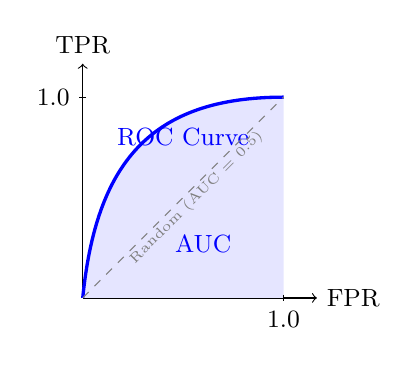
\begin{tikzpicture}[scale=0.85]
            \draw[->] (0,0) -- (3.5,0) node[right, font=\small] {FPR};
            \draw[->] (0,0) -- (0,3.5) node[above, font=\small] {TPR};
            
            \fill[blue!10] (0,0) .. controls (0.2,2.0) and (1.0,3.0) .. (3.0,3.0) -- (3.0,0) -- cycle;
            
            \draw[blue, very thick] (0,0) .. controls (0.2,2.0) and (1.0,3.0) .. (3.0,3.0);
            \node[blue, font=\small] at (1.5,2.4) {ROC Curve};
            
            \draw[dashed, gray] (0,0) -- (3.0,3.0);
            \node[gray, rotate=45, font=\tiny] at (1.7,1.5) {Random (AUC = 0.5)};
            
            \draw (3.0,0.05) -- (3.0,-0.05) node[below, font=\small] {1.0};
            \draw (0.05,3.0) -- (-0.05,3.0) node[left, font=\small] {1.0};
            \node[blue, font=\small] at (1.8,0.8) {AUC};
        \end{tikzpicture}
        \caption{Đường cong ROC tương ứng.}
    \end{subfigure}
    \caption{Trực quan hoá Bipartite Ranking. (a) Ngưỡng $\theta$ phân chia scoring function cảm sinh False Positive (FP) và True Positive (TP). (b) Diện tích tô xanh nhạt dưới đường cong ROC chính là chỉ số AUC.}
    \label{fig:bipartite_roc_concept}
\end{figure}

\begin{example}[Tính AUC bằng tay]
Giả sử có 3 mẫu tích cực với scores $(0.9, 0.7, 0.4)$ và 3 mẫu tiêu cực với scores $(0.8, 0.5, 0.3)$. Để tính toán theo thuật toán của giáo trình Mohri (trang 256), ta tiến hành sắp xếp mảng gộp theo thứ tự **tăng dần (increasing order)**:
\[
    \underbrace{0.3}_{-}, \underbrace{0.4}_{+}, \underbrace{0.5}_{-}, \underbrace{0.7}_{+}, \underbrace{0.8}_{-}, \underbrace{0.9}_{+}.
\]
Ta khởi tạo số lượng phần tử tiêu cực đã duyệt $n_{\text{neg}} = 0$ và số lượng cặp xếp đúng tích lũy $r = 0$. Duyệt mảng từ trái sang phải:
\begin{enumerate}
    \item Gặp $0.3 \ (-)$: là mẫu tiêu cực $\implies n_{\text{neg}} \leftarrow n_{\text{neg}} + 1 = 1$.
    \item Gặp $0.4 \ (+)$: là mẫu tích cực $\implies r \leftarrow r + n_{\text{neg}} = 0 + 1 = 1$.
    \item Gặp $0.5 \ (-)$: là mẫu tiêu cực $\implies n_{\text{neg}} \leftarrow n_{\text{neg}} + 1 = 2$.
    \item Gặp $0.7 \ (+)$: là mẫu tích cực $\implies r \leftarrow r + n_{\text{neg}} = 1 + 2 = 3$.
    \item Gặp $0.8 \ (-)$: là mẫu tiêu cực $\implies n_{\text{neg}} \leftarrow n_{\text{neg}} + 1 = 3$.
    \item Gặp $0.9 \ (+)$: là mẫu tích cực $\implies r \leftarrow r + n_{\text{neg}} = 3 + 3 = 6$.
\end{enumerate}
Tổng số cặp tích dương-tiêu cực: $mn = 3 \times 3 = 9$. Chỉ số AUC thu được là:
\[
    \mathrm{AUC} = \frac{r}{mn} = \frac{6}{9} \approx 0.667.
\]
Kết quả này khớp chính xác tuyệt đối với việc liệt kê và đếm thủ công các cặp $(z'_i, z_j)$ thỏa mãn $h(z'_i) \ge h(z_j)$, bao gồm: $(0.9, 0.8)$, $(0.9, 0.5)$, $(0.9, 0.3)$, $(0.7, 0.5)$, $(0.7, 0.3)$ và $(0.4, 0.3)$ (tổng cộng $6$ cặp).
\end{example}

\begin{extension}
\textbf{Chứng minh Bổ đề phụ: Hướng giảm nhanh nhất của Bipartite RankBoost (Directional Derivative).}

Trong Bipartite RankBoost, mỗi vòng boosting tìm kiếm một base ranker $h_t$ thỏa mãn tối đa hóa hiệu các kỳ vọng $\E_{D^+_t}[h(x')] - \E_{D^-_t}[h(x)]$. Ở đây chúng tôi trình bày chứng minh toán học đầy đủ chỉ ra rằng việc chọn $h_t$ như trên chính là hướng giảm nhanh nhất (cực tiểu directional derivative) của hàm loss bipartite.

Hàm mục tiêu bipartite RankBoost lồi cần tối thiểu hóa là:
\[
    F(\bm{\alpha}) = \sum_{i=1}^m \sum_{j=1}^n \exp\Bigl(-\bigl[f(x'_i) - f(x_j)\bigr]\Bigr),
\]
với $f = \sum_{k=1}^N \alpha_k h_k$. Đạo hàm theo hướng của $F(\bm{\alpha}_{t-1})$ dọc theo tọa độ đơn vị $e_k$ tương ứng với base ranker $h_k$ được định nghĩa:
\[
    F'(\bm{\alpha}_{t-1}; e_k) = \lim_{\eta \to 0} \frac{F(\bm{\alpha}_{t-1} + \eta e_k) - F(\bm{\alpha}_{t-1})}{\eta}.
\]

Tính trực tiếp bằng cách lấy đạo hàm riêng theo $\eta$ tại $\eta = 0$:
\[
    F'(\bm{\alpha}_{t-1}; e_k) = -\sum_{i=1}^m \sum_{j=1}^n \bigl(h_k(x'_i) - h_k(x_j)\bigr) \exp\Bigl(-\bigl[f_{t-1}(x'_i) - f_{t-1}(x_j)\bigr]\Bigr).
\]

Sử dụng đẳng thức phân phối \eqref{eq:D_t1_identity} cho cặp $(i,j)$ tại vòng $t$ với hệ số chuẩn hoá tích lũy $Z_{\text{accum}} = mn \prod_{s=1}^{t-1} Z_s$:
\[
    D_t(i, j) = \frac{\exp\bigl(-[f_{t-1}(x'_i) - f_{t-1}(x_j)]\bigr)}{Z_{\text{accum}}} \implies \exp\Bigl(-\bigl[f_{t-1}(x'_i) - f_{t-1}(x_j)\bigr]\Bigr) = Z_{\text{accum}} D_t(i, j).
\]

Thay vào biểu thức đạo hàm:
\begin{align*}
    F'(\bm{\alpha}_{t-1}; e_k) &= -Z_{\text{accum}} \sum_{i=1}^m \sum_{j=1}^n D_t(i, j) \bigl(h_k(x'_i) - h_k(x_j)\bigr) \\
    &= -Z_{\text{accum}} \sum_{i=1}^m \sum_{j=1}^n D^+_t(i) D^-_t(j) \bigl(h_k(x'_i) - h_k(x_j)\bigr) \quad (\text{do phân phối tách độc lập}) \\
    &= -Z_{\text{accum}} \left[ \sum_{i=1}^m D^+_t(i) h_k(x'_i) \sum_{j=1}^n D^-_t(j) - \sum_{i=1}^m D^+_t(i) \sum_{j=1}^n D^-_t(j) h_k(x_j) \right].
\end{align*}

Do $D^+_t$ và $D^-_t$ là các phân phối xác suất hợp lệ nên tổng của chúng bằng $1$: $\sum_{i=1}^m D^+_t(i) = 1$ và $\sum_{j=1}^n D^-_t(j) = 1$. Thay các tổng này vào:
\begin{align*}
    F'(\bm{\alpha}_{t-1}; e_k) &= -Z_{\text{accum}} \left[ \sum_{i=1}^m D^+_t(i) h_k(x'_i) \cdot 1 - 1 \cdot \sum_{j=1}^n D^-_t(j) h_k(x_j) \right] \\
    &= -Z_{\text{accum}} \left[ \E_{i \sim D^+_t}[h_k(x'_i)] - \E_{j \sim D^-_t}[h_k(x_j)] \right].
\end{align*}

Để cực tiểu hóa đạo hàm theo hướng $F'(\bm{\alpha}_{t-1}; e_k)$ (tức là đi theo hướng giảm nhanh nhất của hàm loss), ta cần **cực đại hóa hiệu các kỳ vọng**:
\[
    \E_{i \sim D^+_t}[h_k(x'_i)] - \E_{j \sim D^-_t}[h_k(x_j)] = \epsilon^+_t - \epsilon^-_t.
\]
Đây chính xác là tiêu chí chọn base ranker $h_t$ trong thuật toán BipartiteRankBoost, hoàn thiện chứng minh toán học cho thuật toán tối ưu.
\end{extension}

\subsubsection{Mối liên hệ học thuật AdaBoost $\leftrightarrow$ RankBoost}

Với định nghĩa $F^+(\bm{\alpha})$ và $F^-(\bm{\alpha})$ như ở \eqref{eq:F_factor}, hàm mục tiêu tối ưu hóa toàn cục của AdaBoost nhị phân có thể được biểu diễn như sau:
\begin{equation}
    F_{\text{AdaBoost}}(\bm{\alpha}) = \sum_{i=1}^m e^{-f(x'_i)} + \sum_{j=1}^n e^{f(x_j)} = F^+(\bm{\alpha}) + F^-(\bm{\alpha}).
\end{equation}
Véc-tơ gradient của hai mô hình có quan hệ hữu cơ:
\begin{equation}
    \nabla F_{\text{RankBoost}} = F^- \nabla F_{\text{AdaBoost}} + (F^+ - F^-)\nabla F^-.
    \label{eq:grad_relation}
\end{equation}

\subsubsection*{Đẳng thức và tính chất giới hạn học thuật}

\begin{tcolorbox}[colback=blue!5, colframe=blue!50!black, title={\textbf{Mối liên hệ học thuật AdaBoost $\leftrightarrow$ RankBoost}}]
Giả sử không gian giả thuyết $\mathcal{H}$ chứa hàm hằng $h_0(x) \equiv 1$. Xét hàm mục tiêu được tối ưu trên tập dữ liệu phân hoạch phi tuyến (non-linearly separable dataset). 
Nếu $(f_s)_{s=1}^\infty$ là một chuỗi các hàm số nằm trong nón của không gian giả thuyết $\Hcal$ sao cho:
\begin{equation}
    \lim_{s \to \infty} F_{\text{AdaBoost}}(f_s) = \inf_{f} F_{\text{AdaBoost}}(f),
\end{equation}
thì chuỗi này cũng đạt cực tiểu tiệm cận cho hàm mục tiêu RankBoost:
\begin{equation}
    \lim_{s \to \infty} F_{\text{RankBoost}}(f_s) = \inf_{f} F_{\text{RankBoost}}(f).
\end{equation}

\textbf{Ý nghĩa học thuật:}
Do $\Hcal$ chứa hàm hằng $h_0 \equiv 1$, tại điểm tiệm cận infimum của AdaBoost, đạo hàm riêng theo trọng số $\alpha_0$ của hàm hằng phải triệt tiêu:
\[
    \frac{\partial F_{\text{AdaBoost}}}{\partial \alpha_0} = 0 \iff -e^{-\alpha_0} F^+ + e^{\alpha_0} F^- = 0 \iff F^+ = F^- \quad (\text{với } \alpha_0 \to 0).
\]
Thế hệ thức cân bằng biên $F^+ = F^-$ vào phương trình gradient liên hệ \eqref{eq:grad_relation}, ta lập tức thu được:
\[
    \nabla F_{\text{RankBoost}}(f_s) \to F^- \cdot \bm{0} + \bm{0} = \bm{0}.
\]
Điều này chứng tỏ điểm tiệm cận của AdaBoost cũng chính là cực trị tiệm cận của RankBoost.

Mặc dù AdaBoost có năng lực tối ưu hóa RankBoost gián tiếp thông qua mối quan hệ toán học này và thường đạt hiệu năng xếp hạng rất tốt trên thực tế, giáo trình Mohri (trang 255) chỉ ra rằng **RankBoost có xu hướng hội tụ nhanh hơn** và đạt chỉ số ranking tối ưu chỉ với ít vòng lặp boosting hơn so với AdaBoost.
\end{tcolorbox}

\begin{extension}
\textbf{Phát biểu nghiêm ngặt về chuỗi Infimum trong không gian phi tuyến}

Giáo trình Mohri đưa ra phát biểu phân tích tiệm cận hết sức cẩn trọng bằng cách sử dụng giới hạn của chuỗi giả thuyết $(f_s)$ và giá trị infimum ($\inf$), thay vì giả định sự tồn tại của một điểm cực tiểu cục bộ duy nhất (minimizer). 

Lý do là trên tập dữ liệu phân hoạch phi tuyến, hàm tổn thất exponential loss của boosting có xu hướng giảm dần về infimum khi các trọng số $\alpha_t$ tiến ra vô cùng (tương tự như hiện tượng phân tách hoàn hảo lề của SVM). Do đó, điểm tối ưu thực tế có thể không tồn tại dưới dạng một véc-tơ hữu hạn, và việc phát biểu bằng chuỗi tiệm cận toán học là bắt buộc để đảm bảo tính đúng đắn và chặt chẽ của lý thuyết chứng minh.
\end{extension}

\begin{extension}
\textbf{Hạn chế học thuật của AUC: Ví dụ phản chứng về sự tương đương hiệu năng.}

Mặc dù AUC là một chỉ số cực kỳ phổ biến trong bipartite ranking, nó có một hạn chế học thuật rất lớn: **AUC tính trung bình trên toàn bộ đường cong ROC**, điều này có thể dẫn đến việc đánh giá sai lệch hiệu năng trong thực tế.

Xét hai mô hình xếp hạng $A$ và $B$ trên cùng một tập dữ liệu. Đường cong ROC của chúng giao nhau:
\begin{itemize}
    \item **Mô hình A**: Đạt True Positive Rate (TPR) rất cao khi False Positive Rate (FPR) nhỏ (ví dụ: TPR = $0.70$ tại FPR = $0.05$), nhưng tăng chậm ở giai đoạn sau.
    \item **Mô hình B**: Đạt TPR rất thấp khi FPR nhỏ (ví dụ: TPR = $0.20$ tại FPR = $0.05$), nhưng tăng rất nhanh ở giai đoạn sau.
\end{itemize}
Giả sử cả hai mô hình đều có diện tích dưới đường cong ROC bằng nhau: $\text{AUC}(A) = \text{AUC}(B) = 0.80$. 

\textbf{Ví dụ phản chứng cho sự tương đương hiệu năng:}
\begin{enumerate}
    \item Trong bài toán **truy hồi thông tin (Information Retrieval / Search Engine)**: Người dùng chỉ quan tâm đến các kết quả ở trang đầu tiên (tương ứng với vùng FPR cực kỳ nhỏ ở góc dưới bên trái của đường ROC). Tại vùng này, mô hình $A$ vượt trội hoàn toàn so với mô hình $B$ (TPR $0.70$ so với $0.20$). Tuy nhiên, chỉ số AUC của chúng lại bằng nhau ($0.80$), khiến ta lầm tưởng hai mô hình có giá trị sử dụng ngang nhau.
    \item Trong bài toán **phát hiện giao dịch gian lận (Fraud Detection)**: Nhân viên điều tra chỉ có thể kiểm tra một số lượng rất ít giao dịch nghi vấn mỗi ngày do giới hạn nguồn lực. Do đó, mô hình phải có khả năng gom các giao dịch gian lận lên top đầu của danh sách (FPR cực thấp). Mô hình $A$ là sự lựa chọn duy nhất khả thi, trong khi mô hình $B$ hoàn toàn vô dụng trên thực tế.
\end{enumerate}

Sự bất cập này của chỉ số AUC là động lực chính để các nhà nghiên cứu chuyển sang sử dụng các tiêu chí xếp hạng khác tập trung vào phần đầu danh sách, chẳng hạn như **Normalized Discounted Cumulative Gain (NDCG)** hoặc chỉ số **Partial AUC** (chỉ tính diện tích đường ROC từ FPR = $0$ đến một ngưỡng $\beta$ cụ thể).
\end{extension}

% ── KHẢO SÁT MỐI LIÊN HỆ LÝ THUYẾT ────────────────────────────────────────────
\subsubsection{Khảo sát mối liên hệ học thuật với các chương khác trong giáo trình}
\label{sec:connections}

Để hoàn thành trọn vẹn Yêu cầu số 5 của đề tài đồ án về việc ``Khảo sát mối liên hệ giữa các nội dung lý thuyết'', chúng tôi tiến hành phân tích sâu sắc các kết nối toán học hữu cơ giữa nội dung phân hạng (Chương 10) với các chương nền tảng khác trong cuốn sách \textit{Foundations of Machine Learning}:

\paragraph{1. RankBoost $\leftrightarrow$ AdaBoost (Kết nối với Chương 7 - Boosting)}
* **Sự thống nhất về hàm tổn thất**: RankBoost thực chất là sự mở rộng của thuật toán AdaBoost (Chương 7) từ việc học trên từng điểm mẫu đơn lẻ (pointwise) sang học trên các cặp thực thể (pairwise). Cả hai thuật toán đều cực tiểu hóa cận trên lồi dạng hàm mũ ($e^{-u}$) của hàm tổn thất gốc (Zero-One loss).
* **Sự tương đương về mặt thuật toán**: Quy trình tối ưu của RankBoost chính là phương pháp hạ độ dốc tọa độ (Coordinate Descent) trên hàm mục tiêu lồi $F(\bm{\alpha})$, hoàn toàn tương thích với cơ chế tối ưu của AdaBoost. Hơn nữa, phân tích tiệm cận của Mohri chỉ ra rằng nếu tập base rankers chứa hàm hằng, AdaBoost nhị phân chuẩn cũng sẽ hội tụ về điểm tối ưu tiệm cận của RankBoost trong không gian bipartite.

\paragraph{2. Chặn sai số RankBoost $\leftrightarrow$ Rademacher Complexity (Kết nối với Chương 3 - Generalization Bounds)}
* **Cơ sở đo lường năng lực học tập**: Sai số phân hạng thực tế $R(h)$ được chặn trên thông qua Rademacher Complexity của không gian giả thuyết $\Hcal$ theo Định lý 10.2 và Hệ quả 10.4. Độ phức tạp Rademacher (định nghĩa tại Chương 3) đóng vai trò đo lường khả năng khớp nhiễu ngẫu nhiên của tập giả thuyết $\Hcal$.
* **Sự phân tách Rademacher trong Bipartite**: Khác với phân loại nhị phân thông thường (chỉ có một số hạng Rademacher trên tập mẫu chung), chặn lề phân hạng nhị phân phân tách độ phức tạp Rademacher thành hai thành phần riêng biệt $R^{D^+}_m(\Hcal)$ và $R^{D^-}_n(\Hcal)$ tương ứng trên không gian mẫu dương $S^+$ (kích thước $m$) và mẫu âm $S^-$ (kích thước $n$). Đây là điểm tinh tế toán học cực kỳ quan trọng: trong khi Corollary 10.4 tổng quát dùng chung kích thước mẫu $m$ cho cả hai số hạng Rademacher (do chọn mẫu theo cặp), thì trong bipartite setting cụ thể, ta có $m$ mẫu tích cực độc lập từ $D^+$ và $n$ mẫu tiêu cực độc lập từ $D^-$, dẫn đến hai Rademacher terms sử dụng độc lập hai sample sizes khác nhau là $m$ và $n$.

\paragraph{3. Bipartite Setting $\leftrightarrow$ Binary Classification (Kết nối với Chương 3 \& 7)}
* **Cực tiểu sai số phân hạng bằng phân loại nhị phân**: Bipartite ranking có thể được rút gọn một phần về bài toán phân loại nhị phân bằng cách gán ngưỡng tuyệt đối $\theta$. Sai số phân hạng thực tế $R(h)$ có thể được chặn trên thông qua sai số phân loại nhị phân:
  \begin{equation}
      R(h) \leq 2 R_{\text{class}}(h).
  \end{equation}
  Đây là kết quả lý thuyết quan trọng được nêu tại **Bài tập 10.7 (Exercise 10.7)** của giáo trình Mohri, chứng minh rằng một bộ phân lớp hoạt động tốt chắc chắn sẽ đảm bảo sai số phân hạng thấp.
* **Sự ưu việt của phân hạng trên dữ liệu mất cân bằng**: Khác với phân loại nhị phân (nơi các chỉ số Accuracy hay F1-score cực kỳ nhạy cảm và dễ bị bóp méo khi tập dữ liệu bị mất cân bằng nghiêm trọng), độ đo phân hạng AUC hoàn toàn bất biến (invariant) trước sự thay đổi tỷ lệ số lượng giữa mẫu dương ($m$) và mẫu âm ($n$). Điều này chứng minh tại sao phương pháp phân hạng bipartite (như BipartiteRankBoost) luôn được ưu tiên lựa chọn thay thế cho classification trong các ứng dụng thực tế mất cân bằng dữ liệu như Search Engine hay Fraud Detection.
